\PassOptionsToPackage{unicode=true}{hyperref} % options for packages loaded elsewhere
\PassOptionsToPackage{hyphens}{url}
%
\documentclass[portuguese,]{article}
\usepackage{lmodern}
\usepackage{amssymb,amsmath}
\usepackage{ifxetex,ifluatex}
\usepackage{fixltx2e} % provides \textsubscript
\ifnum 0\ifxetex 1\fi\ifluatex 1\fi=0 % if pdftex
  \usepackage[T1]{fontenc}
  \usepackage[utf8]{inputenc}
  \usepackage{textcomp} % provides euro and other symbols
\else % if luatex or xelatex
  \usepackage{unicode-math}
  \defaultfontfeatures{Ligatures=TeX,Scale=MatchLowercase}
\fi
% use upquote if available, for straight quotes in verbatim environments
\IfFileExists{upquote.sty}{\usepackage{upquote}}{}
% use microtype if available
\IfFileExists{microtype.sty}{%
\usepackage[]{microtype}
\UseMicrotypeSet[protrusion]{basicmath} % disable protrusion for tt fonts
}{}
\IfFileExists{parskip.sty}{%
\usepackage{parskip}
}{% else
\setlength{\parindent}{0pt}
\setlength{\parskip}{6pt plus 2pt minus 1pt}
}
\usepackage{hyperref}
\hypersetup{
            pdftitle={Folha 1, Ex. 2 --- Estutura Electrónica e Modelação Computacional},
            pdfauthor={Miguel Murça, 2015235874},
            pdfborder={0 0 0},
            breaklinks=true}
\urlstyle{same}  % don't use monospace font for urls
\usepackage{color}
\usepackage{fancyvrb}
\newcommand{\VerbBar}{|}
\newcommand{\VERB}{\Verb[commandchars=\\\{\}]}
\DefineVerbatimEnvironment{Highlighting}{Verbatim}{commandchars=\\\{\}}
% Add ',fontsize=\small' for more characters per line
\newenvironment{Shaded}{}{}
\newcommand{\AlertTok}[1]{\textcolor[rgb]{1.00,0.00,0.00}{\textbf{#1}}}
\newcommand{\AnnotationTok}[1]{\textcolor[rgb]{0.38,0.63,0.69}{\textbf{\textit{#1}}}}
\newcommand{\AttributeTok}[1]{\textcolor[rgb]{0.49,0.56,0.16}{#1}}
\newcommand{\BaseNTok}[1]{\textcolor[rgb]{0.25,0.63,0.44}{#1}}
\newcommand{\BuiltInTok}[1]{#1}
\newcommand{\CharTok}[1]{\textcolor[rgb]{0.25,0.44,0.63}{#1}}
\newcommand{\CommentTok}[1]{\textcolor[rgb]{0.38,0.63,0.69}{\textit{#1}}}
\newcommand{\CommentVarTok}[1]{\textcolor[rgb]{0.38,0.63,0.69}{\textbf{\textit{#1}}}}
\newcommand{\ConstantTok}[1]{\textcolor[rgb]{0.53,0.00,0.00}{#1}}
\newcommand{\ControlFlowTok}[1]{\textcolor[rgb]{0.00,0.44,0.13}{\textbf{#1}}}
\newcommand{\DataTypeTok}[1]{\textcolor[rgb]{0.56,0.13,0.00}{#1}}
\newcommand{\DecValTok}[1]{\textcolor[rgb]{0.25,0.63,0.44}{#1}}
\newcommand{\DocumentationTok}[1]{\textcolor[rgb]{0.73,0.13,0.13}{\textit{#1}}}
\newcommand{\ErrorTok}[1]{\textcolor[rgb]{1.00,0.00,0.00}{\textbf{#1}}}
\newcommand{\ExtensionTok}[1]{#1}
\newcommand{\FloatTok}[1]{\textcolor[rgb]{0.25,0.63,0.44}{#1}}
\newcommand{\FunctionTok}[1]{\textcolor[rgb]{0.02,0.16,0.49}{#1}}
\newcommand{\ImportTok}[1]{#1}
\newcommand{\InformationTok}[1]{\textcolor[rgb]{0.38,0.63,0.69}{\textbf{\textit{#1}}}}
\newcommand{\KeywordTok}[1]{\textcolor[rgb]{0.00,0.44,0.13}{\textbf{#1}}}
\newcommand{\NormalTok}[1]{#1}
\newcommand{\OperatorTok}[1]{\textcolor[rgb]{0.40,0.40,0.40}{#1}}
\newcommand{\OtherTok}[1]{\textcolor[rgb]{0.00,0.44,0.13}{#1}}
\newcommand{\PreprocessorTok}[1]{\textcolor[rgb]{0.74,0.48,0.00}{#1}}
\newcommand{\RegionMarkerTok}[1]{#1}
\newcommand{\SpecialCharTok}[1]{\textcolor[rgb]{0.25,0.44,0.63}{#1}}
\newcommand{\SpecialStringTok}[1]{\textcolor[rgb]{0.73,0.40,0.53}{#1}}
\newcommand{\StringTok}[1]{\textcolor[rgb]{0.25,0.44,0.63}{#1}}
\newcommand{\VariableTok}[1]{\textcolor[rgb]{0.10,0.09,0.49}{#1}}
\newcommand{\VerbatimStringTok}[1]{\textcolor[rgb]{0.25,0.44,0.63}{#1}}
\newcommand{\WarningTok}[1]{\textcolor[rgb]{0.38,0.63,0.69}{\textbf{\textit{#1}}}}
\usepackage{longtable,booktabs}
% Fix footnotes in tables (requires footnote package)
\IfFileExists{footnote.sty}{\usepackage{footnote}\makesavenoteenv{longtable}}{}
\usepackage{graphicx,grffile}
\makeatletter
\def\maxwidth{\ifdim\Gin@nat@width>\linewidth\linewidth\else\Gin@nat@width\fi}
\def\maxheight{\ifdim\Gin@nat@height>\textheight\textheight\else\Gin@nat@height\fi}
\makeatother
% Scale images if necessary, so that they will not overflow the page
% margins by default, and it is still possible to overwrite the defaults
% using explicit options in \includegraphics[width, height, ...]{}
\setkeys{Gin}{width=\maxwidth,height=\maxheight,keepaspectratio}
\setlength{\emergencystretch}{3em}  % prevent overfull lines
\providecommand{\tightlist}{%
  \setlength{\itemsep}{0pt}\setlength{\parskip}{0pt}}
\setcounter{secnumdepth}{5}
% Redefines (sub)paragraphs to behave more like sections
\ifx\paragraph\undefined\else
\let\oldparagraph\paragraph
\renewcommand{\paragraph}[1]{\oldparagraph{#1}\mbox{}}
\fi
\ifx\subparagraph\undefined\else
\let\oldsubparagraph\subparagraph
\renewcommand{\subparagraph}[1]{\oldsubparagraph{#1}\mbox{}}
\fi

% set default figure placement to htbp
\makeatletter
\def\fps@figure{htbp}
\makeatother

\usepackage{supertabular, listings, physics}
\lstset{
    basicstyle=\small,
    frame=single
}
\makeatletter
\def\fps@figure{h}
\makeatother
\ifnum 0\ifxetex 1\fi\ifluatex 1\fi=0 % if pdftex
  \usepackage[shorthands=off,main=portuguese]{babel}
\else
  % load polyglossia as late as possible as it *could* call bidi if RTL lang (e.g. Hebrew or Arabic)
  \usepackage{polyglossia}
  \setmainlanguage[]{portuguese}
\fi

\title{Folha 1, Ex. 2 --- Estutura Electrónica e Modelação Computacional}
\author{Miguel Murça, 2015235874}
\date{}

\begin{document}
\maketitle

\hypertarget{energias-de-ionizauxe7uxe3o}{%
\section{Energias de Ionização}\label{energias-de-ionizauxe7uxe3o}}

Recorrendo ao programa de Química Quântica PSI4, começou por se
calcular, recorrendo ao método de Hartree-Fock na base STO-3G, a energia
total das moléculas de H2 e HeH+para distâncias de ligação variáveis
(\ref{code:vardist}).

Os pontos \texttt{(d,\ E)} obtidos encontram-se apresentados em
\ref{data:varH} e \ref{data:varHeH}. A representação gráfica dos pontos
encontra-se nas figuras \ref{fig:varH} e \ref{fig:varHeH}

\begin{figure}
\centering
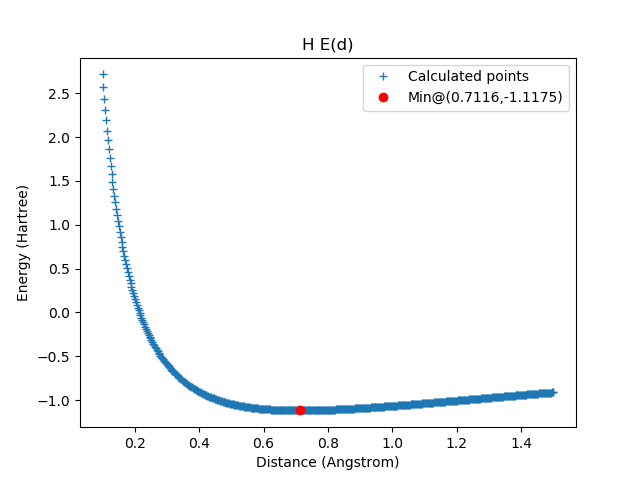
\includegraphics{bits/figures/ex2-H.png}
\caption{Gráfico d(E) dos valores obtidos para a energia total da
molécula de Hidrogénio, de acordo com o método de Hartree-Fock, na base
STO-3G. Foi calculada a energia para 500 pontos, uniformemente espaçados
entre 0.1\AA e 1.5\AA. \label{fig:varH}}
\end{figure}

\begin{figure}
\centering
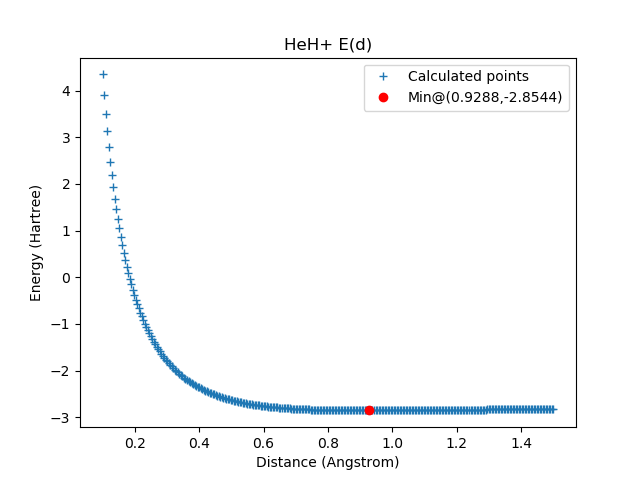
\includegraphics{bits/figures/ex2-HeH.png}
\caption{Gráfico d(E) dos valores obtidos para a energia total da
molécula HeH+, de acordo com o método de Hartree-Fock, na base STO-3G.
Foi calculada a energia para 300 pontos, uniformemente espaçados entre
0.1\AA e 1.5\AA. \label{fig:varHeH}}
\end{figure}

Simultaneamente ao cálculo dos pontos apresentados, identificaram-se
também os pontos de energia total mínima:

\[ \text{Distância de Energia Mínima}_{\text{H}_2}   = d_{\text{H}_2}   = \left ( 0.7116 \, , \, -1.1175 \right ) \]

\[ \text{Distância de Energia Mínima}_{\text{HeH}^+} = d_{\text{HeH}^+} = \left ( 0.9288 \, , \, -2.8522 \right ) \]

Tomando as estas distâncias, determinaram-se, recorrendo de novo ao
programa PSI4, as propriedades das moléculas onde a distância de ligação
é igual à distância de energia mínima.

Os excertos relevantes do \emph{output} obtido encontram-se apresentados
nas figuras \ref{output:Hmin} e \ref{output:HeHmin}

\begin{figure}[htb]
\begin{lstlisting}
...
set basis sto-3g
...
energy('scf', molecule=H)
...
    Orbital Energies [Eh]
    ---------------------

    Doubly Occupied:                                                      

       1Ag    -0.590501  

    Virtual:                                                              

       1B1u    0.701093  

    Final Occupation by Irrep:
             Ag   B1g   B2g   B3g    Au   B1u   B2u   B3u 
    DOCC [     1,    0,    0,    0,    0,    0,    0,    0 ]

    Energy converged.

    @DF-RHF Final Energy:    -1.11752981987458
...
\end{lstlisting}
\caption{Excertos relevantes do output produzido pelo PSI4 para H2}
\label{output:Hmin}
\end{figure}

\begin{figure}[htb]
\begin{lstlisting}
...
set basis sto-3g
...
energy('scf', molecule=HeH)
...
    Orbital Energies [Eh]
    ---------------------

    Doubly Occupied:                                                      

       1A1    -1.524298  

    Virtual:                                                              

       2A1    -0.267229  

    Final Occupation by Irrep:
             A1    A2    B1    B2 
    DOCC [     1,    0,    0,    0 ]


    Energy converged.

    @DF-RHF Final Energy:    -2.85441846621746
...
\end{lstlisting}
\caption{Excertos relevantes do output produzido pelo PSI4 para HeH+}
\label{output:HeHmin}
\end{figure}

Nestes estão indicadas as energias HOMO para cada espécie, nomeadamente:

\[ \epsilon^{\text{H}_2}_{\text{HOMO}}   = -0.590501 \quad \text{(Hartree)} \]

\[ \epsilon^{\text{HeH}^+}_{\text{HOMO}} = -1.270649 \quad \text{(Hartree)} \]

Assim como a energia total de cada espécie:

\[ \text{E}^{\text{H}_2} = -1.117530 \quad \text{(Hartree)} \]

\[ \text{E}^{\text{HeH}^+} = -2.854418 \quad \text{(Hartree)} \]

De acordo com o teorema de Koopmans, a energia de ionização \(I_p\) de
uma espécie química com energia da HOMO \(\epsilon_\text{HOMO}\) é dada
por

\[ I_p = - \epsilon_\text{HOMO} \]

Este teorema assume que a contribuição da relaxação da orbital da
espécie ionizada para a energia total é desprezável face a \(\epsilon\),
ou seja, assume que as orbitais de \(\ket{{}^N \Psi_0}\) são óptimas
para o estado \(\ket{{}^{N-1} \Psi_a}\). Esta aproximação pode ser
designada por aproximação de ``orbitais congeladas''. Desprezada a
diminuição da energia pela relaxação, esperar-se-ia que a energia
prevista para a ionização da espécie fosse inferior (em módulo) à
energia experimentalmente verificada, mas é necessário ter em conta que
se \(\epsilon_\text{HOMO}\) for obtido pelo método de Hartree-Fock, o
termo de troca é perdido, pelo que a energia obtida no cálculo direto da
espécie ionizada (onde a relaxação é contabilizada) pode não ser
inferior (em módulo) à energia total obtida para a espécie não-ionizada.

Para verificar estas observações, calcularam-se, de novo recorrendo ao
PSI4 com o método de (\emph{Unrestricted}) Hartree-Fock na base STO-3G
(\textbf{UHF/STO-3G}), as energias totais para \(\text{H}_2^+\) e
\(\text{HeH}^{2+}\) (mantendo as respetivas distâncias de ligação
internuclear \(d_{\text{H}_2}\) e \(d_{\text{HeH}^+}\)). Os ficheiros de
input descrevendo as moléculas para uso no PSI4 encontram-se
apresentados na secção \ref{code:ioninp}.

Os excertos relevantes do \emph{output} obtido encontram-se apresentados
nas figuras \ref{output:Hion}, \ref{output:HeHion}.

\begin{figure}[htb]
\begin{lstlisting}
    Alpha Occupied:                                                       

       1Ag    -1.270649  

    Alpha Virtual:                                                        

       1B1u    0.032566  

    Beta Occupied:                                                        

    

    Beta Virtual:                                                         

       1Ag    -0.590501     1B1u    0.212115  

    Final Occupation by Irrep:
             Ag   B1g   B2g   B3g    Au   B1u   B2u   B3u 
    DOCC [     0,    0,    0,    0,    0,    0,    0,    0 ]
    SOCC [     1,    0,    0,    0,    0,    0,    0,    0 ]

  Energy converged.

  @DF-UHF Final Energy:    -0.52702876420193
...
\end{lstlisting}
\caption{Excertos relevantes do output produzido pelo PSI4 para $H_2^+$}
\label{output:Hion}
\end{figure}

\begin{figure}[htb]
\begin{lstlisting}
    Alpha Occupied:                                                       

       1A1    -2.497832  

    Alpha Virtual:                                                        

       2A1    -0.837902  

    Beta Occupied:                                                        

    

    Beta Virtual:                                                         

       1A1    -1.480189     2A1    -0.751747  

    Final Occupation by Irrep:
             A1    A2    B1    B2 
    DOCC [     0,    0,    0,    0 ]
    SOCC [     1,    0,    0,    0 ]

  Energy converged.

  @DF-UHF Final Energy:    -1.35666548775990
...
\end{lstlisting}
\caption{Excertos relevantes do output produzido pelo PSI4 para $HeH^{2+}$}
\label{output:HeHion}
\end{figure}

A energia total das espécies ionizada é então, de acordo com UHF/STO-3G:

\[ \text{E}_{\text{H}_2^+} = -0.527029 \quad \text{(Hartree)} \]

\[ \text{E}_{\text{HeH}^{2+}} = -1.356665 \quad \text{(Hartree)} \]

Encontra-se, na tabela \ref{tab:ionenergies}, comparada a energia de
ionização obtida pelo teorema de Koopmans (\(I_p\)) com a energia de
ionização prevista por aplicação direta de UHF/STO-3G (\(I_d\)), assim
como com energias de ionização experimentalmente previstas (NIST, 2018)
(\(I_e\)).

\begin{longtable}[]{@{}lllll@{}}
\caption{Comparação das energias HOMO (\(\epsilon\)), total (E), e
energias de ionização pelo teorema de Koopmans (\(I_p\)) e por cálculo
da energia da espécie ionizada (\(I_d\)). Todos os valores estão
expressos em Hartree. Os valores \(E\) e \(\epsilon\) foram obtidos por
cálculo com UHF/STO-3G. \label{tab:ionenergies}}\tabularnewline
\toprule
& \(H_2\) & \(HeH^+\) & \(H_2^+\) & \(HeH^{2+}\)\tabularnewline
\midrule
\endfirsthead
\toprule
& \(H_2\) & \(HeH^+\) & \(H_2^+\) & \(HeH^{2+}\)\tabularnewline
\midrule
\endhead
E & -1.117553 & -2.854418 & -0.527029 & -1.356665\tabularnewline
\(\epsilon\) & -0.590501 & -1.270649 & --- & ---\tabularnewline
\(I_p\) & 0.590501 & 1.270649 & --- & ---\tabularnewline
\(I_d\) & 0.590524 & 1.497753 & --- & ---\tabularnewline
\(I_e\) & 0.566895 & Sem Dados & --- & ---\tabularnewline
\bottomrule
\end{longtable}

\pagebreak

Observa-se que para o \(H_2\) as energias de ionização \(I_p\) e \(I_d\)
concordam em quatro casas decimais, pelo que a energia de relaxação
electrónica pode, de facto, ser desprezada em boa aproximação. Isto é
esperado, uma vez que o número de electrões na espécie original
(\(H_2\)) é muito reduzido, pelo que a energia de relaxação é pequena.

No entanto, observa-se que tanto \(I_p\) como \(I_d\) apenas concordam
com \(I_e\) na primeira casa decimal; está presente um erro sistemático
que poderá advir da escolha da base. Recorrendo a UHF/cc-pVTZ (cujo
input para o PSI4 se encontra apresentado em \ref{code:ccpvtz} com
output \ref{output:ccpvtz}), observam-se os resultados apresentados na
tabela \ref{tab:ccpvtz}.

\begin{longtable}[]{@{}lllll@{}}
\caption{Valores obtidos para energia total (E), energia HOMO
(\(\epsilon\)), energia de ionização a partir do teorema de Koopmans
(\(I_p\)) e energia de ionização por cálculo da energia total da espécie
ionizada (\(I_d\)), recorrendo a \textbf{URH/cc-pVTZ}.
\label{tab:ccpvtz}}\tabularnewline
\toprule
& \(H_2\) & \(HeH^+\) & \(H_2^+\) & \(HeH^{2+}\)\tabularnewline
\midrule
\endfirsthead
\toprule
& \(H_2\) & \(HeH^+\) & \(H_2^+\) & \(HeH^{2+}\)\tabularnewline
\midrule
\endhead
E & -1,132599 & -2.923252 & -0.560512 & -1.447928\tabularnewline
\(\epsilon\) & -0.603595 & -1.528449 & --- & ---\tabularnewline
\(I_p\) & 0.603595 & 1.528449 & --- & ---\tabularnewline
\(I_d\) & 0.572087 & 1.475324 & --- & ---\tabularnewline
\bottomrule
\end{longtable}

Verifica-se que em comparação com a tabela \ref{tab:ionenergies}, a
energia de ionização \(I_d\) obtida encontra-se mais próxima da energia
experimentalmente verificada.

Para \(\text{HeH}^+\) a carga nuclear é mais elevada, pelo que a energia
de relaxação deve ser mais elevada. Observa-se, de facto, que nesse caso
\(I_p\) e \(I_d\) já são discordantes na primeira casa decimal.

\hypertarget{energia-de-dissociauxe7uxe3o}{%
\section{Energia de Dissociação}\label{energia-de-dissociauxe7uxe3o}}

Para verificar qual a energia total dos sistemas (de acordo com
UHF/STO-3G) no regime de distância internuclear tão grande que se podem
considerar átomos separados, calcularam-se as energias totais para
distâncias exponencialmente crescentes, observando o valor energético
assimptótico. Os resultados obtidos encontram-se apresentados nas
figuras \ref{fig:Hassimp}, \ref{fig:HeHassimp}.

\begin{figure}
\centering
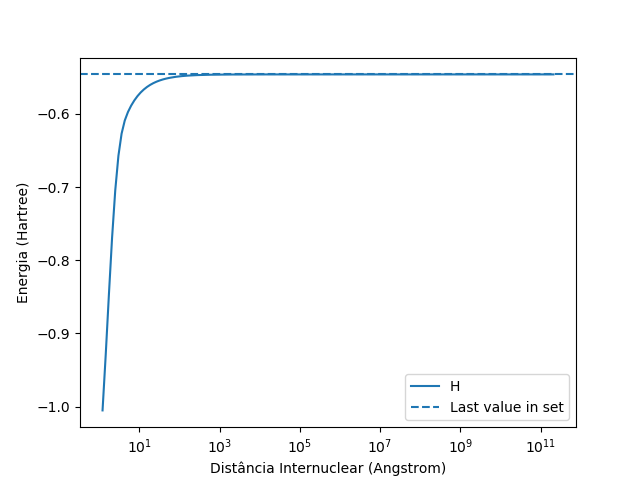
\includegraphics{bits/figures/H.png}
\caption{Valores de energia total da molécula H2 (de acordo com
UHF/STO-3G) para distâncias internucleares exponencialmente crescentes.
\label{fig:Hassimp}}
\end{figure}

\begin{figure}
\centering
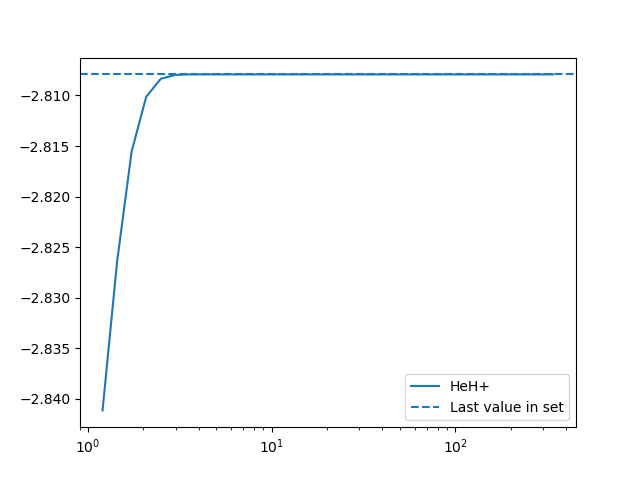
\includegraphics{bits/figures/HeH+.png}
\caption{Valores de energia total da molécula de HeH+ (de acordo com
UHF/STO-3G) para distâncias internucleares exponencialmente crescentes.
\label{fig:HeHassimp}}
\end{figure}

Observa-se que para distâncias da ordem de \(10^4\) e superior as
moléculas apresentam comportamento assimptótico.

Neste regime, as energias totais das moléculas são (de acrodo com
UHF/STO-3G),

\[ \text{E}_{\text{H}_2}    = -0.546008 \quad \text{(Hartree)} \]

\[ \text{E}_{\text{HeH}^+}  = -2.807913 \quad \text{(Hartree)} \]

Calculou-se a energia dos átomos/iões individuais em UHF/STO-3G,
obtendo-se os resultados apresentados na tabela \ref{tab:atoms}.

\begin{longtable}[]{@{}ll@{}}
\caption{Valores obtidos (UHF/STO-3G) para a energia total dos átomos e
respetivos iões nas moléculas de H2 e HeH+.
\label{tab:atoms}}\tabularnewline
\toprule
\endhead
\begin{minipage}[t]{0.13\columnwidth}\raggedright
Espécie\strut
\end{minipage} & \begin{minipage}[t]{0.35\columnwidth}\raggedright
Energia Total (Hartree)\strut
\end{minipage}\tabularnewline
\begin{minipage}[t]{0.13\columnwidth}\raggedright
H\strut
\end{minipage} & \begin{minipage}[t]{0.35\columnwidth}\raggedright
-0.466582\strut
\end{minipage}\tabularnewline
\begin{minipage}[t]{0.13\columnwidth}\raggedright
H+\strut
\end{minipage} & \begin{minipage}[t]{0.35\columnwidth}\raggedright
-0.000000\strut
\end{minipage}\tabularnewline
\begin{minipage}[t]{0.13\columnwidth}\raggedright
H-\strut
\end{minipage} & \begin{minipage}[t]{0.35\columnwidth}\raggedright
-0.158852\strut
\end{minipage}\tabularnewline
\begin{minipage}[t]{0.13\columnwidth}\raggedright
He\strut
\end{minipage} & \begin{minipage}[t]{0.35\columnwidth}\raggedright
-2.807913\strut
\end{minipage}\tabularnewline
\begin{minipage}[t]{0.13\columnwidth}\raggedright
He+\strut
\end{minipage} & \begin{minipage}[t]{0.35\columnwidth}\raggedright
-1.931748\strut
\end{minipage}\tabularnewline
\bottomrule
\end{longtable}

Considerando as possíveis dissociações de H2 e respetivas energias
(calculadas pela soma das energias das espécies dissociadas):

\begin{minipage}{\textwidth}

$\textbf{H}_2$

\quad $E_\text{Grande Distância} = -0.546008 \quad \text{(Hartree)}$

\qquad $H_2 \longrightarrow H + H$

\qquad \quad $\sum E = -0.933164 \quad \text{(Hartree)}$

\qquad $H_2 \longrightarrow H^+ + H^-$

\qquad \quad $\sum E = -0.158852 \quad \text{(Hartree)}$

\end{minipage}

\begin{minipage}{\textwidth}

$\textbf{HeH}^+$

\quad $E_\text{Grande Distância} = -2.807913 \quad \text{(Hartree)}$

\qquad $HeH^{+} \longrightarrow He + H^+$

\qquad \quad $\sum E = -2.807913 \quad \text{(Hartree)}$

\qquad $HeH^{+} \longrightarrow He^+ + H$

\qquad \quad $\sum E = -2.3983303 \quad \text{(Hartree)}$

\end{minipage}

\hypertarget{referuxeancias}{%
\section{Referências}\label{referuxeancias}}

NIST Computational Chemistry Comparison and Benchmark Database,\\
NIST Standard Reference Database Number 101\\
Release 19, April 2018, Editor: Russell D. Johnson III\\
http://cccbdb.nist.gov/

\begin{center}\rule{0.5\linewidth}{\linethickness}\end{center}

\twocolumn
\appendix

\hypertarget{raw-data}{%
\section{\texorpdfstring{\emph{Raw Data}}{Raw Data}}\label{raw-data}}

\hypertarget{h2}{%
\subsection{H2}\label{h2}}

\label{data:varH}

\begingroup
\tiny
\tablehead{Internuclear \\
    Distance (Angstrom) & E (Hartree) \\ }
\begin{supertabular}{ll}
0.1                 & 2.715809425962524     \\
0.1028056112224449  & 2.573362550671971     \\
0.10561122244488978 & 2.4386349108468877    \\
0.10841683366733468 & 2.311030221836967     \\
0.11122244488977956 & 2.190012294191016     \\
0.11402805611222445 & 2.0750976399229923    \\
0.11683366733466935 & 1.9658491441571417    \\
0.11963927855711423 & 1.8618706272639907    \\
0.12244488977955913 & 1.7628021546596466    \\
0.12525050100200402 & 1.6683159770334637    \\
0.1280561122244489  & 1.5781130043190195    \\
0.13086172344689379 & 1.4919197333046839    \\
0.13366733466933867 & 1.409485562231918     \\
0.13647294589178358 & 1.3305804366906122    \\
0.13927855711422846 & 1.254992780094836     \\
0.14208416833667337 & 1.1825276694037714    \\
0.14488977955911825 & 1.1130052228434626    \\
0.14769539078156313 & 1.0462591714393432    \\
0.150501002004008   & 0.9821355903721349    \\
0.15330661322645292 & 0.9204917696820333    \\
\end{supertabular} \tablehead{}
\begin{supertabular}{ll}
0.1561122244488978  & 0.8611952067898966    \\
0.15891783567134268 & 0.8041227057795756    \\
0.1617234468937876  & 0.7491595704760032    \\
0.16452905811623247 & 0.6961988801214902    \\
0.16733466933867736 & 0.6451408379547442    \\
0.17014028056112224 & 0.5958921842767042    \\
0.17294589178356712 & 0.5483656666783772    \\
0.17575150300601203 & 0.5024795610426147    \\
0.17855711422845694 & 0.4581572377333639    \\
0.18136272545090182 & 0.41532676807868363   \\
0.1841683366733467  & 0.373920566848457     \\
0.18697394789579158 & 0.33387506694591396   \\
0.18977955911823646 & 0.29513042297730163   \\
0.19258517034068137 & 0.25763024075336904   \\
0.19539078156312625 & 0.2213213301165673    \\
0.19819639278557116 & 0.1861534787790704    \\
0.20100200400801604 & 0.15207924511927973   \\
0.20380761523046093 & 0.11905376810848867   \\
0.2066132264529058  & 0.08703459273760072   \\
0.2094188376753507  & 0.05598150948957137   \\
\end{supertabular}
\begin{supertabular}{ll}
0.2122244488977956  & 0.025856406557309253  \\
0.21503006012024048 & -0.00337686635954082  \\
0.2178356713426854  & -0.031752623722357876 \\
0.22064128256513027 & -0.059303460225931026 \\
0.22344689378757515 & -0.08606035811894197  \\
0.22625250501002003 & -0.11205278653393236  \\
0.22905811623246494 & -0.13730879351198866  \\
0.23186372745490982 & -0.16185509134275766  \\
0.2346693386773547  & -0.18571713577969484  \\
0.23747494989979961 & -0.20891919963756134  \\
0.2402805611222445  & -0.231484441233076    \\
0.24308617234468938 & -0.25343496808538557  \\
0.24589178356713426 & -0.27479189625617984  \\
0.24869739478957917 & -0.29557540567447393  \\
0.251503006012024   & -0.31580479176004383  \\
0.25430861723446896 & -0.33549851363265304  \\
0.25711422845691384 & -0.35467423916797514  \\
0.2599198396793587  & -0.37334888713929615  \\
0.2627254509018036  & -0.3915386666637447   \\
0.2655310621242485  & -0.4092591141525779   \\
\end{supertabular}
\begin{supertabular}{ll}
0.2683366733466934  & -0.4265251279489891   \\
0.27114228456913825 & -0.4433510008214563   \\
0.2739478957915832  & -0.45975045046685814  \\
0.27675350701402807 & -0.47573664816512584  \\
0.27955911823647295 & -0.4913222457153448   \\
0.28236472945891783 & -0.5065194007740197   \\
0.2851703406813627  & -0.5213398007053699   \\
0.28797595190380765 & -0.5357946850452056   \\
0.2907815631262525  & -0.549894866673549    \\
0.2935871743486974  & -0.5636507517813071   \\
0.2963927855711423  & -0.5770723587120808   \\
0.2991983967935872  & -0.5901693357529771   \\
0.30200400801603206 & -0.6029509779427288   \\
0.30480961923847694 & -0.6154262429614075   \\
0.3076152304609219  & -0.6276037661594814   \\
0.3104208416833667  & -0.6394918747818528   \\
0.31322645290581164 & -0.6510986014368955   \\
0.3160320641282565  & -0.6624316968577021   \\
0.3188376753507014  & -0.6734986419993035   \\
0.3216432865731463  & -0.6843066595124091   \\
\end{supertabular}
\begin{supertabular}{ll}
0.32444889779559116 & -0.694862724631627    \\
0.3272545090180361  & -0.7051735755129805   \\
0.3300601202404809  & -0.715245723053987    \\
0.33286573146292586 & -0.7250854602267702   \\
0.33567134268537074 & -0.7346988709520352   \\
0.3384769539078156  & -0.7440918385416628   \\
0.34128256513026056 & -0.7532700537337311   \\
0.3440881763527054  & -0.7622390223435526   \\
0.3468937875751503  & -0.7710040725527367   \\
0.34969939879759515 & -0.779570361855732    \\
0.3525050100200401  & -0.787942883683769    \\
0.355310621242485   & -0.7961264737231946   \\
0.35811623246492985 & -0.804125815945268    \\
0.3609218436873748  & -0.8119454483629481   \\
0.3637274549098196  & -0.8195897685291509   \\
0.36653306613226455 & -0.8270630387903117   \\
0.3693386773547094  & -0.8343693913081358   \\
0.3721442885771543  & -0.8415128328615475   \\
0.37494989979959925 & -0.8484972494403386   \\
0.3777555110220441  & -0.8553264106410263   \\
\end{supertabular}
\begin{supertabular}{ll}
0.380561122244489   & -0.8620039738750758   \\
0.38336673346693384 & -0.8685334883988641   \\
0.3861723446893788  & -0.8749183991745376   \\
0.3889779559118236  & -0.8811620505696248   \\
0.39178356713426854 & -0.887267689903845    \\
0.3945891783567135  & -0.8932384708502881   \\
0.3973947895791583  & -0.8990774566979151   \\
0.40020040080160324 & -0.9047876234823106   \\
0.40300601202404807 & -0.9103718629905364   \\
0.405811623246493   & -0.9158329856463434   \\
0.40861723446893783 & -0.9211737232811539   \\
0.41142284569138277 & -0.9263967317960683   \\
0.4142284569138277  & -0.9315045937200673   \\
0.41703406813627253 & -0.936499820668737    \\
0.41983967935871747 & -0.9413848557085785   \\
0.4226452905811623  & -0.946162075630671    \\
0.42545090180360723 & -0.9508337931375992   \\
0.42825651302605205 & -0.9554022589480746   \\
0.431062124248497   & -0.9598696638221792   \\
0.43386773547094193 & -0.9642381405110382   \\
\end{supertabular}
\begin{supertabular}{ll}
0.43667334669338675 & -0.9685097656339228   \\
0.4394789579158317  & -0.9726865614862151   \\
0.4422845691382765  & -0.9767704977806819   \\
0.44509018036072145 & -0.9807634933252449   \\
0.4478957915831663  & -0.9846674176397396   \\
0.4507014028056112  & -0.9884840925139678   \\
0.45350701402805615 & -0.9922152935099893   \\
0.456312625250501   & -0.9958627514102234   \\
0.4591182364729459  & -0.9994281536140334   \\
0.46192384769539074 & -1.0029131454846842   \\
0.4647294589178357  & -1.006319331648744    \\
0.4675350701402805  & -1.0096482772494864   \\
0.47034068136272544 & -1.012901509156566    \\
0.4731462925851704  & -1.0160805171332434   \\
0.4759519038076152  & -1.0191867549630391   \\
0.47875751503006014 & -1.0222216415373162   \\
0.48156312625250497 & -1.0251865619051992   \\
0.4843687374749499  & -1.0280828682873788   \\
0.48717434869739473 & -1.0309118810550126   \\
0.48997995991983967 & -1.0336748896751868   \\
\end{supertabular}
\begin{supertabular}{ll}
0.4927855711422846  & -1.0363731536240839   \\
0.49559118236472943 & -1.0390079032689759   \\
0.49839679358717437 & -1.0415803407204458   \\
0.5012024048096192  & -1.0440916406554983   \\
0.5040080160320641  & -1.0465429511131579   \\
0.5068136272545091  & -1.0489353942630322   \\
0.5096192384769539  & -1.051270067148124    \\
0.5124248496993988  & -1.0535480424028192   \\
0.5152304609218437  & -1.0557703689466185   \\
0.5180360721442886  & -1.0579380726549603   \\
0.5208416833667334  & -1.0600521570074986   \\
0.5236472945891784  & -1.0621136037149028   \\
0.5264529058116233  & -1.0641233733248177   \\
0.5292585170340681  & -1.0660824058077676   \\
0.5320641282565131  & -1.0679916211236344   \\
0.5348697394789579  & -1.0698519197694971   \\
0.5376753507014028  & -1.0716641833093306   \\
0.5404809619238476  & -1.0734292748863377   \\
0.5432865731462926  & -1.0751480397184467   \\
0.5460921843687375  & -1.0768213055774691   \\
\end{supertabular}
\begin{supertabular}{ll}
0.5488977955911823  & -1.0784498832527372   \\
0.5517034068136273  & -1.0800345669993754   \\
0.5545090180360721  & -1.0815761349722055   \\
0.557314629258517   & -1.0830753496451773   \\
0.5601202404809619  & -1.0845329582175713   \\
0.5629258517034068  & -1.0859496930066264   \\
0.5657314629258517  & -1.087326271827697    \\
0.5685370741482966  & -1.088663398362017    \\
0.5713426853707415  & -1.0899617625126865   \\
0.5741482965931863  & -1.0912220407490698   \\
0.5769539078156313  & -1.0924448964401512   \\
0.5797595190380761  & -1.09363098017735     \\
0.582565130260521   & -1.094780930086821    \\
0.585370741482966   & -1.0958953721318823   \\
0.5881763527054108  & -1.0969749204057955   \\
0.5909819639278557  & -1.0980201774153517   \\
0.5937875751503006  & -1.0990317343552496   \\
0.5965931863727455  & -1.1000101713740995   \\
0.5993987975951903  & -1.1009560578318665   \\
0.6022044088176353  & -1.1018699525493272   \\
\end{supertabular}
\begin{supertabular}{ll}
0.6050100200400801  & -1.1027524040497076   \\
0.607815631262525   & -1.1036039507928377   \\
0.61062124248497    & -1.1044251214019973   \\
0.6134268537074148  & -1.105216434883812    \\
0.6162324649298597  & -1.1059784008414377   \\
0.6190380761523046  & -1.1067115196810455   \\
0.6218436873747495  & -1.1074162828122318   \\
0.6246492985971943  & -1.1080931728422976   \\
0.6274549098196393  & -1.108742663764584    \\
0.6302605210420842  & -1.10936522114131     \\
0.633066132264529   & -1.1099613022809232   \\
0.635871743486974   & -1.1105313564101307   \\
0.6386773547094188  & -1.1110758248409898   \\
0.6414829659318637  & -1.11159514113307     \\
0.6442885771543085  & -1.1120897312509497   \\
0.6470941883767535  & -1.1125600137171283   \\
0.6498997995991984  & -1.1130063997606712   \\
0.6527054108216432  & -1.1134292934615688   \\
0.6555110220440882  & -1.113829091891073    \\
0.658316633266533   & -1.1142061852481957   \\
\end{supertabular}
\begin{supertabular}{ll}
0.6611222444889779  & -1.1145609569923536   \\
0.6639278557114228  & -1.114893783972472    \\
0.6667334669338677  & -1.1152050365525668   \\
0.6695390781563126  & -1.1154950787339875   \\
0.6723446893787575  & -1.1157642682744573   \\
0.6751503006012024  & -1.1160129568039214   \\
0.6779559118236472  & -1.1162414899375555   \\
0.6807615230460922  & -1.1164502073856513   \\
0.683567134268537   & -1.1166394430610185   \\
0.6863727454909819  & -1.116809525183498    \\
0.6891783567134269  & -1.1169607763819847   \\
0.6919839679358717  & -1.1170935137940057   \\
0.6947895791583166  & -1.1172080491628098   \\
0.6975951903807615  & -1.1173046889323657   \\
0.7004008016032064  & -1.1173837343398996   \\
0.7032064128256512  & -1.1174454815065145   \\
0.7060120240480962  & -1.117490221525678    \\
0.7088176352705411  & -1.117518240549742    \\
0.7116232464929859  & -1.1175298198745847   \\
0.7144288577154309  & -1.1175252360224446   \\
\end{supertabular}
\begin{supertabular}{ll}
0.7172344689378757  & -1.1175047608229103   \\
0.7200400801603206  & -1.1174686614923859   \\
0.7228456913827654  & -1.117417200711772    \\
0.7256513026052104  & -1.1173506367025774   \\
0.7284569138276553  & -1.1172692233016834   \\
0.7312625250501001  & -1.117173210034407    \\
0.7340681362725451  & -1.117062842186385    \\
0.7368737474949899  & -1.116938360873971    \\
0.7396793587174348  & -1.1168000031133034   \\
0.7424849699398797  & -1.1166480018882083   \\
0.7452905811623246  & -1.116482586216799    \\
0.7480961923847695  & -1.1163039812169733   \\
0.7509018036072144  & -1.1161124081706753   \\
0.7537074148296593  & -1.1159080845871132   \\
0.7565130260521041  & -1.1156912242649164   \\
0.7593186372745491  & -1.1154620373532216   \\
0.762124248496994   & -1.1152207304118433   \\
0.7649298597194388  & -1.1149675064703652   \\
0.7677354709418838  & -1.1147025650863878   \\
0.7705410821643286  & -1.1144261024027107   \\
\end{supertabular}
\begin{supertabular}{ll}
0.7733466933867735  & -1.1141383112039551   \\
0.7761523046092184  & -1.113839380971874    \\
0.7789579158316633  & -1.1135294979403192   \\
0.7817635270541082  & -1.1132088451488988   \\
0.7845691382765531  & -1.1128776024962854   \\
0.787374749498998   & -1.11253594679247     \\
0.7901803607214428  & -1.1121840518103738   \\
0.7929859719438878  & -1.1118220883366898   \\
0.7957915831663326  & -1.1114502242220672   \\
0.7985971943887775  & -1.1110686244305459   \\
0.8014028056112225  & -1.1106774510882804   \\
0.8042084168336673  & -1.1102768635316669   \\
0.8070140280561122  & -1.1098670183547479   \\
0.809819639278557   & -1.1094480694560254   \\
0.812625250501002   & -1.109020168084611    \\
0.8154308617234468  & -1.1085834628857592   \\
0.8182364729458917  & -1.108138099945815    \\
0.8210420841683367  & -1.1076842228364512   \\
0.8238476953907815  & -1.1072219726585488   \\
0.8266533066132264  & -1.106751488085198    \\
\end{supertabular}
\begin{supertabular}{ll}
0.8294589178356713  & -1.1062729054044      \\
0.8322645290581162  & -1.1057863585610206   \\
0.835070140280561   & -1.1052919791982432   \\
0.837875751503006   & -1.1047898966984642   \\
0.8406813627254509  & -1.1042802382236885   \\
0.8434869739478957  & -1.103763128755316    \\
0.8462925851703407  & -1.1032386911334053   \\
0.8490981963927855  & -1.1027070460954675   \\
0.8519038076152304  & -1.1021683123147106   \\
0.8547094188376753  & -1.1016226064376524   \\
0.8575150300601202  & -1.1010700431214553   \\
0.8603206412825651  & -1.100510735070463    \\
0.86312625250501    & -1.0999447930725117   \\
0.8659318637274549  & -1.0993723260345518   \\
0.8687374749498997  & -1.0987934410177942   \\
0.8715430861723447  & -1.0982082432724276   \\
0.8743486973947895  & -1.0976168362718421   \\
0.8771543086172344  & -1.0970193217462616   \\
0.8799599198396794  & -1.096415799715953    \\
0.8827655310621242  & -1.0958063685240806   \\
\end{supertabular}
\begin{supertabular}{ll}
0.8855711422845691  & -1.095191124868791    \\
0.888376753507014   & -1.0945701638350802   \\
0.8911823647294589  & -1.093943578926134    \\
0.8939879759519038  & -1.0933114620940128   \\
0.8967935871743486  & -1.0926739037701232   \\
0.8995991983967936  & -1.0920309928950946   \\
0.9024048096192384  & -1.0913828169481445   \\
0.9052104208416833  & -1.0907294619761052   \\
0.9080160320641282  & -1.0900710126219155   \\
0.9108216432865731  & -1.0894075521526176   \\
0.913627254509018   & -1.088739162487014    \\
0.9164328657314629  & -1.088065924222778    \\
0.9192384769539078  & -1.0873879166631486   \\
0.9220440881763526  & -1.0867052178431693   \\
0.9248496993987976  & -1.0860179045555123   \\
0.9276553106212424  & -1.0853260523758244   \\
0.9304609218436873  & -1.0846297356876762   \\
0.9332665330661323  & -1.0839290277069922   \\
0.9360721442885771  & -1.0832240005061933   \\
0.938877755511022   & -1.0825147250377516   \\
\end{supertabular}
\begin{supertabular}{ll}
0.9416833667334669  & -1.081801271157456    \\
0.9444889779559118  & -1.0810837076471267   \\
0.9472945891783566  & -1.080362102237058    \\
0.9501002004008016  & -1.0796365216278743   \\
0.9529058116232465  & -1.0789070315121516   \\
0.9557114228456913  & -1.0781736965954558   \\
0.9585170340681363  & -1.0774365806171469   \\
0.9613226452905811  & -1.0766957463706022   \\
0.964128256513026   & -1.0759512557232251   \\
0.9669338677354709  & -1.075203169635899    \\
0.9697394789579158  & -1.0744515481821475   \\
0.9725450901803607  & -1.0736964505668896   \\
0.9753507014028056  & -1.0729379351447603   \\
0.9781563126252505  & -1.0721760594381293   \\
0.9809619238476953  & -1.0714108801546973   \\
0.9837675350701403  & -1.0706424532047198   \\
0.9865731462925851  & -1.0698708337178835   \\
0.98937875751503    & -1.069096076059778    \\
0.992184368737475   & -1.0683182338481467   \\
0.9949899799599198  & -1.067537359968561    \\
\end{supertabular}
\begin{supertabular}{ll}
0.9977955911823647  & -1.066753506589905    \\
1.0006012024048097  & -1.0659667251794926   \\
1.0034068136272545  & -1.0651770665178097   \\
1.0062124248496993  & -1.064384580712924    \\
1.0090180360721444  & -1.0635893172145985   \\
1.0118236472945892  & -1.0627913248280438   \\
1.014629258517034   & -1.0619906517273794   \\
1.017434869739479   & -1.0611873454686709   \\
1.0202404809619239  & -1.0603814530028937   \\
1.0230460921843687  & -1.0595730206882696   \\
1.0258517034068135  & -1.0587620943026144   \\
1.0286573146292586  & -1.057948719055097    \\
1.0314629258517034  & -1.057132939597997    \\
1.0342685370741482  & -1.0563148000379303   \\
1.0370741482965933  & -1.0554943439468691   \\
1.039879759519038   & -1.0546716143729915   \\
1.042685370741483   & -1.0538466538510467   \\
1.045490981963928   & -1.0530195044127186   \\
1.0482965931863728  & -1.0521902075964364   \\
1.0511022044088176  & -1.051358804457112    \\
\end{supertabular}
\begin{supertabular}{ll}
1.0539078156312625  & -1.050525335575657    \\
1.0567134268537075  & -1.0496898410680244   \\
1.0595190380761523  & -1.0488523605943139   \\
1.0623246492985972  & -1.048012933367347    \\
1.0651302605210422  & -1.047171598161204    \\
1.067935871743487   & -1.0463283933194503   \\
1.0707414829659319  & -1.0454833567631512   \\
1.0735470941883767  & -1.0446365259986794   \\
1.0763527054108217  & -1.0437879381252722   \\
1.0791583166332666  & -1.042937629842411    \\
1.0819639278557114  & -1.0420856374570153   \\
1.0847695390781564  & -1.04123199689035     \\
1.0875751503006013  & -1.0403767436848437   \\
1.090380761523046   & -1.0395199130106398   \\
1.093186372745491   & -1.0386615396719527   \\
1.095991983967936   & -1.0378016581133487   \\
1.0987975951903808  & -1.0369403024257267   \\
1.1016032064128256  & -1.036077506352131    \\
1.1044088176352707  & -1.03521330329351     \\
1.1072144288577155  & -1.034347726314192    \\
\end{supertabular}
\begin{supertabular}{ll}
1.1100200400801603  & -1.0334808081472406   \\
1.1128256513026054  & -1.0326125811996756   \\
1.1156312625250502  & -1.0317430775574947   \\
1.118436873747495   & -1.0308723289905877   \\
1.12124248496994    & -1.0300003669574864   \\
1.1240480961923849  & -1.0291272226099926   \\
1.1268537074148297  & -1.0282529267976601   \\
1.1296593186372745  & -1.0273775100720735   \\
1.1324649298597196  & -1.0265010026911838   \\
1.1352705410821644  & -1.0256234346232995   \\
1.1380761523046092  & -1.0247448355510793   \\
1.1408817635270543  & -1.0238652348754624   \\
1.143687374749499   & -1.0229846617192804   \\
1.146492985971944   & -1.0221031449310214   \\
1.1492985971943888  & -1.0212207130882418   \\
1.1521042084168338  & -1.0203373945010652   \\
1.1549098196392786  & -1.019453217215445    \\
1.1577154308617235  & -1.0185682090164478   \\
1.1605210420841685  & -1.0176823974313227   \\
1.1633266533066133  & -1.0167958097325833   \\
\end{supertabular}
\begin{supertabular}{ll}
1.1661322645290582  & -1.0159084729409391   \\
1.168937875751503   & -1.0150204138281598   \\
1.171743486973948   & -1.0141316589198872   \\
1.1745490981963929  & -1.0132422344983296   \\
1.1773547094188377  & -1.0123521666048725   \\
1.1801603206412827  & -1.0114614810426414   \\
1.1829659318637276  & -1.0105702033790456   \\
1.1857715430861724  & -1.0096783589481166   \\
1.1885771543086172  & -1.0087859728529218   \\
1.1913827655310623  & -1.0078930699678195   \\
1.194188376753507   & -1.006999674940727    \\
1.196993987975952   & -1.0061058121952475   \\
1.199799599198397   & -1.0052115059328415   \\
1.2026052104208418  & -1.0043167801348498   \\
1.2054108216432866  & -1.003421658564513    \\
1.2082164328657314  & -1.0025261647689403   \\
1.2110220440881765  & -1.0016303220810339   \\
1.2138276553106213  & -1.0007341536213472   \\
1.2166332665330661  & -0.9998376822998959   \\
1.2194388777555112  & -0.9989409308179872   \\
\end{supertabular}
\begin{supertabular}{ll}
1.222244488977956   & -0.9980439216699125   \\
1.2250501002004008  & -0.9971466771446932   \\
1.2278557114228457  & -0.9962492193277255   \\
1.2306613226452907  & -0.9953515701024335   \\
1.2334669338677355  & -0.9944537511518496   \\
1.2362725450901804  & -0.9935557839602134   \\
1.2390781563126254  & -0.9926576898144917   \\
1.2418837675350702  & -0.9917594898058713   \\
1.244689378757515   & -0.9908612048312795   \\
1.24749498997996    & -0.9899628555948119   \\
1.250300601202405   & -0.9890644626091857   \\
1.2531062124248498  & -0.9881660461971101   \\
1.2559118236472946  & -0.9872676264927179   \\
1.2587174348697396  & -0.9863692234428704   \\
1.2615230460921845  & -0.9854708568085848   \\
1.2643286573146293  & -0.9845725461662437   \\
1.2671342685370741  & -0.9836743109089985   \\
1.2699398797595192  & -0.9827761702479899   \\
1.272745490981964   & -0.9818781432136514   \\
1.2755511022044088  & -0.9809802486569427   \\
\end{supertabular}
\begin{supertabular}{ll}
1.2783567134268539  & -0.9800825052506165   \\
1.2811623246492987  & -0.97918493149038     \\
1.2839679358717435  & -0.9782875456961724   \\
1.2867735470941883  & -0.977390366013324    \\
1.2895791583166334  & -0.9764934104137689   \\
1.2923847695390782  & -0.9755966966971606   \\
1.295190380761523   & -0.974700242492085    \\
1.297995991983968   & -0.973804065257203    \\
1.300801603206413   & -0.9729081822823824   \\
1.3036072144288577  & -0.9720126106898119   \\
1.3064128256513026  & -0.9711173674351578   \\
1.3092184368737476  & -0.970222469308663    \\
1.3120240480961924  & -0.9693279329362395   \\
1.3148296593186373  & -0.9684337747805857   \\
1.3176352705410823  & -0.9675400111422643   \\
1.3204408817635271  & -0.9666466581607941   \\
1.323246492985972   & -0.9657537318157147   \\
1.3260521042084168  & -0.9648612479276814   \\
1.3288577154308618  & -0.9639692221594927   \\
1.3316633266533067  & -0.9630776700171843   \\
\end{supertabular}
\begin{supertabular}{ll}
1.3344689378757515  & -0.9621866068510718   \\
1.3372745490981965  & -0.9612960478567779   \\
1.3400801603206414  & -0.9604060080763127   \\
1.3428857715430862  & -0.9595165023990795   \\
1.345691382765531   & -0.9586275455629294   \\
1.348496993987976   & -0.9577391521551707   \\
1.351302605210421   & -0.9568513366136141   \\
1.3541082164328657  & -0.9559641132275852   \\
1.3569138276553108  & -0.955077496138915    \\
1.3597194388777556  & -0.9541914993430185   \\
1.3625250501002004  & -0.9533061366898237   \\
1.3653306613226452  & -0.952421421884825    \\
1.3681362725450903  & -0.9515373684900813   \\
1.3709418837675351  & -0.9506539899251987   \\
1.37374749498998    & -0.9497712994683288   \\
1.376553106212425   & -0.9488893102571503   \\
1.3793587174348698  & -0.9480080352898818   \\
1.3821643286573146  & -0.947127487426235    \\
1.3849699398797595  & -0.9462476793884146   \\
1.3877755511022045  & -0.9453686237621065   \\
\end{supertabular}
\begin{supertabular}{ll}
1.3905811623246493  & -0.9444903329973799   \\
1.3933867735470942  & -0.9436128194097556   \\
1.3961923847695392  & -0.9427360951811157   \\
1.398997995991984   & -0.9418601723606548   \\
1.4018036072144289  & -0.9409850628658805   \\
1.404609218436874   & -0.9401107784835409   \\
1.4074148296593187  & -0.9392373308705894   \\
1.4102204408817636  & -0.9383647315551235   \\
1.4130260521042084  & -0.9374929919373337   \\
1.4158316633266534  & -0.9366221232904379   \\
1.4186372745490983  & -0.9357521367616516   \\
1.421442885771543   & -0.9348830433730737   \\
1.4242484969939881  & -0.934014854022662    \\
1.427054108216433   & -0.9331475794851328   \\
1.4298597194388778  & -0.9322812304128759   \\
1.4326653306613226  & -0.931415817336923    \\
1.4354709418837677  & -0.9305513506677952   \\
1.4382765531062125  & -0.9296878406964897   \\
1.4410821643286573  & -0.9288252975953      \\
1.4438877755511024  & -0.9279637314188084   \\
\end{supertabular}
\begin{supertabular}{ll}
1.4466933867735472  & -0.9271031521047275   \\
1.449498997995992   & -0.9262435694748137   \\
1.4523046092184368  & -0.9253849932357728   \\
1.455110220440882   & -0.9245274329801118   \\
1.4579158316633267  & -0.9236708981870608   \\
1.4607214428857715  & -0.9228153982234328   \\
1.4635270541082166  & -0.9219609423444955   \\
1.4663326653306614  & -0.9211075396948484   \\
1.4691382765531062  & -0.9202551993092902   \\
1.471943887775551   & -0.9194039301136719   \\
1.4747494989979961  & -0.918553740925768    \\
1.477555110220441   & -0.9177046404561072   \\
1.4803607214428858  & -0.9168566373088333   \\
1.4831663326653308  & -0.9160097399825617   \\
1.4859719438877756  & -0.9151639568711755   \\
1.4887775551102205  & -0.9143192962647134   \\
1.4915831663326653  & -0.9134757663501583   \\
1.4943887775551103  & -0.9126333752122673   \\
1.4971943887775552  & -0.9117921308344011   \\
1.5                 & -0.9109520410993436   \\
\end{supertabular}
\endgroup

\hypertarget{heh}{%
\subsection{HeH+}\label{heh}}

\label{data:varHeH}

\begingroup
\tiny
\tiny
\tablehead{Internuclear \\
    Distance (Angstrom) & E (Hartree) \\ }
\begin{supertabular}{ll}
0.1                 & 4.347543874624938    \\
0.10468227424749164 & 3.9026901819387128   \\
0.10936454849498328 & 3.498137937253945    \\
0.11404682274247492 & 3.128843154619932    \\
0.11872909698996656 & 2.7905593302237106   \\
0.1234113712374582  & 2.4796869585837626   \\
0.12809364548494984 & 2.193155841751441    \\
0.13277591973244146 & 1.9283321260412274   \\
0.1374581939799331  & 1.6829441978041513   \\
0.14214046822742477 & 1.4550231144764558   \\
0.1468227424749164  & 1.2428543479311212   \\
0.15150501672240801 & 1.0449384115178801   \\
0.15618729096989967 & 0.8599585221424442   \\
0.16086956521739132 & 0.6867538768557044   \\
0.16555183946488294 & 0.5242974427227216   \\
0.17023411371237457 & 0.37167739919977905  \\
0.17491638795986622 & 0.22808155498894322  \\
0.17959866220735787 & 0.09278420141560906  \\
0.1842809364548495  & -0.03486502739292163 \\
0.18896321070234112 & -0.15545063297243367 \\
\end{supertabular} \tablehead{}
\begin{supertabular}{ll}
0.19364548494983277 & -0.2694993489925357  \\
0.19832775919732443 & -0.3774870829225494  \\
0.20301003344481605 & -0.47984488862719177 \\
0.20769230769230768 & -0.5769641224925925  \\
0.21237458193979933 & -0.6692009090428757  \\
0.21705685618729098 & -0.7568800204750872  \\
0.2217391304347826  & -0.8402982570450561  \\
0.22642140468227426 & -0.9197274009556138  \\
0.23110367892976588 & -0.9954168046803129  \\
0.2357859531772575  & -1.0675956650150908  \\
0.24046822742474916 & -1.1364750261676926  \\
0.2451505016722408  & -1.2022495485772904  \\
0.24983277591973244 & -1.2650990746410695  \\
0.2545150501672241  & -1.3251900179173666  \\
0.2591973244147157  & -1.3826765985111227  \\
0.26387959866220734 & -1.4377019441001089  \\
0.268561872909699   & -1.4903990733181232  \\
0.2732441471571906  & -1.5408917758970668  \\
0.27792642140468227 & -1.5892954020011614  \\
0.28260869565217395 & -1.6357175715165848  \\
\end{supertabular}
\begin{supertabular}{ll}
0.2872909698996655  & -1.680258812633627   \\
0.2919732441471572  & -1.7230131378401925  \\
0.2966555183946488  & -1.7640685644006524  \\
0.30133779264214045 & -1.80350758549762    \\
0.3060200668896321  & -1.8414075974415487  \\
0.3107023411371237  & -1.8778412876873334  \\
0.3153846153846154  & -1.9128769878205596  \\
0.32006688963210705 & -1.9465789951769734  \\
0.3247491638795986  & -1.9790078663259207  \\
0.3294314381270903  & -2.0102206852712525  \\
0.33411371237458193 & -2.0402713088950257  \\
0.33879598662207355 & -2.0692105918825474  \\
0.34347826086956523 & -2.097086593117247   \\
0.3481605351170568  & -2.1239447653132375  \\
0.3528428093645485  & -2.14982812946206    \\
0.35752508361204016 & -2.1747774354997684  \\
0.36220735785953173 & -2.1988313104520643  \\
0.3668896321070234  & -2.222026395183735   \\
0.371571906354515   & -2.2443974707623546  \\
0.37625418060200666 & -2.2659775753439924  \\
\end{supertabular}
\begin{supertabular}{ll}
0.38093645484949834 & -2.2867981123973338  \\
0.3856187290969899  & -2.306888951002502   \\
0.3903010033444816  & -2.3262785188887416  \\
0.39498327759197327 & -2.34499388881151    \\
0.39966555183946484 & -2.3630608588131707  \\
0.4043478260869565  & -2.3805040268597137  \\
0.4090301003344481  & -2.397346860301955   \\
0.41371237458193977 & -2.4136117605677274  \\
0.41839464882943145 & -2.429320123456219   \\
0.423076923076923   & -2.444492395372575   \\
0.4277591973244147  & -2.459148125811048   \\
0.4324414715719064  & -2.473306016369504   \\
0.43712374581939795 & -2.4869839665532503  \\
0.4418060200668896  & -2.5001991166051423  \\
0.4464882943143812  & -2.512967887579843   \\
0.4511705685618729  & -2.5253060188602103  \\
0.45585284280936456 & -2.537228603302045   \\
0.4605351170568561  & -2.548750120174081   \\
0.4652173913043478  & -2.559884466050298   \\
0.4698996655518395  & -2.5706449837978314  \\
\end{supertabular}
\begin{supertabular}{ll}
0.47458193979933105 & -2.5810444897935465  \\
0.47926421404682273 & -2.591095299491918   \\
0.4839464882943143  & -2.600809251457778   \\
0.488628762541806   & -2.610197729969084   \\
0.49331103678929766 & -2.619271686286952   \\
0.49799331103678923 & -2.6280416586835074  \\
0.5026755852842809  & -2.636517791311061   \\
0.5073578595317726  & -2.6447098519903287  \\
0.5120401337792642  & -2.652627248990105   \\
0.5167224080267558  & -2.6602790468652264  \\
0.5214046822742474  & -2.667673981415211   \\
0.5260869565217391  & -2.6748204738215304  \\
0.5307692307692308  & -2.6817266440173526  \\
0.5354515050167223  & -2.6884003233399065  \\
0.540133779264214   & -2.6948490665120377  \\
0.5448160535117057  & -2.7010801629964107  \\
0.5494983277591973  & -2.7071006477626565  \\
0.554180602006689   & -2.7129173115050413  \\
0.5588628762541805  & -2.718536710345689   \\
0.5635451505016722  & -2.7239651750557323  \\
\end{supertabular}
\begin{supertabular}{ll}
0.5682274247491639  & -2.729208819824871   \\
0.5729096989966554  & -2.734273550607793   \\
0.5775919732441471  & -2.739165073071502   \\
0.5822742474916388  & -2.7438889001730007  \\
0.5869565217391304  & -2.7484503593838356  \\
0.5916387959866221  & -2.752854599586896   \\
0.5963210702341136  & -2.757106597663614   \\
0.6010033444816053  & -2.7612111647899384  \\
0.605685618729097   & -2.7651729524582587  \\
0.6103678929765886  & -2.768996458240978   \\
0.6150501672240802  & -2.772686031310469   \\
0.6197324414715718  & -2.776245877729173   \\
0.6244147157190635  & -2.7796800655225002  \\
0.6290969899665552  & -2.7829925295464064  \\
0.6337792642140467  & -2.7861870761606875  \\
0.6384615384615384  & -2.789267387718212   \\
0.64314381270903    & -2.7922370268797345  \\
0.6478260869565217  & -2.7950994407630274  \\
0.6525083612040133  & -2.7978579649347823  \\
0.6571906354515049  & -2.8005158272529114  \\
\end{supertabular}
\begin{supertabular}{ll}
0.6618729096989966  & -2.803076151566413   \\
0.6665551839464883  & -2.805541961279558   \\
0.6712374581939798  & -2.807916182786659   \\
0.6759197324414715  & -2.8102016487832744  \\
0.6806020066889632  & -2.8124011014591517  \\
0.6852842809364548  & -2.8145171955782864  \\
0.6899665551839465  & -2.8165525014506834  \\
0.694648829431438   & -2.8185095078002105  \\
0.6993311036789297  & -2.8203906245330197  \\
0.7040133779264214  & -2.8221981854102243  \\
0.708695652173913   & -2.823934450628614   \\
0.7133779264214046  & -2.8256016093128826  \\
0.7180602006688962  & -2.827201781922718   \\
0.7227424749163879  & -2.828737022577683   \\
0.7274247491638796  & -2.830209321302975   \\
0.7321070234113711  & -2.83162060619875    \\
0.7367892976588628  & -2.8329727455356903  \\
0.7414715719063545  & -2.8342675497792302  \\
0.7461538461538461  & -2.835506773544801   \\
0.7508361204013377  & -2.836692117486617   \\
\end{supertabular}
\begin{supertabular}{ll}
0.7555183946488294  & -2.837825230121696   \\
0.760200668896321   & -2.838907709591628   \\
0.7648829431438127  & -2.839941105363815   \\
0.7695652173913042  & -2.8409269198741494  \\
0.7742474916387959  & -2.841866610113014   \\
0.7789297658862876  & -2.842761589156183   \\
0.7836120401337792  & -2.843613227642629   \\
0.7882943143812708  & -2.844422855200643   \\
0.7929765886287624  & -2.8451917618237657  \\
0.7976588628762541  & -2.845921199198515   \\
0.8023411371237458  & -2.846612381984826   \\
0.8070234113712373  & -2.8472664890511576  \\
0.811705685618729   & -2.8478846646653517  \\
0.8163879598662207  & -2.848468019642794   \\
0.8210702341137123  & -2.849017632453102   \\
0.825752508361204   & -2.8495345502868004  \\
0.8304347826086956  & -2.850019790083115   \\
0.8351170568561872  & -2.850474339520183   \\
0.8397993311036789  & -2.850899157968954   \\
0.8444816053511705  & -2.8512951774118864  \\
\end{supertabular}
\begin{supertabular}{ll}
0.8491638795986621  & -2.851663303327662   \\
0.8538461538461538  & -2.8520044155430675  \\
0.8585284280936454  & -2.852319369053073   \\
0.8632107023411371  & -2.8526089948103515  \\
0.8678929765886286  & -2.8528741004850735  \\
0.8725752508361203  & -2.853115471196302   \\
0.877257525083612   & -2.8533338702157884  \\
0.8819397993311036  & -2.853530039645229   \\
0.8866220735785952  & -2.853704701068009   \\
0.8913043478260869  & -2.853858556176258   \\
0.8959866220735785  & -2.853992287374334   \\
0.9006688963210702  & -2.8541065583594203  \\
0.9053511705685618  & -2.8542020146802463  \\
0.9100334448160534  & -2.8542792842748375  \\
0.9147157190635451  & -2.8543389779879575  \\
0.9193979933110367  & -2.854381690069181   \\
0.9240802675585283  & -2.854407998652406   \\
0.92876254180602    & -2.8544184662174645  \\
0.9334448160535116  & -2.8544136400346103  \\
0.9381270903010033  & -2.8543940525927463  \\
\end{supertabular}
\begin{supertabular}{ll}
0.9428093645484948  & -2.8543602220118043  \\
0.9474916387959865  & -2.854312652440255   \\
0.9521739130434782  & -2.854251834438208   \\
0.9568561872909698  & -2.8541782453467603  \\
0.9615384615384615  & -2.8540923496443065  \\
0.9662207357859531  & -2.8539945992902838  \\
0.9709030100334447  & -2.85388543405689    \\
0.9755852842809364  & -2.853765281849552   \\
0.9802675585284281  & -2.8536345590163688  \\
0.9849498327759196  & -2.853493670647127   \\
0.9896321070234113  & -2.8533430108626368  \\
0.9943143812709029  & -2.853182963094369   \\
0.9989966555183946  & -2.853013900355248   \\
1.0036789297658864  & -2.8528361855063755  \\
1.0083612040133778  & -2.8526501714931825  \\
1.0130434782608695  & -2.8524562016177764  \\
1.0177257525083612  & -2.852254609760718   \\
1.0224080267558529  & -2.8520457206169016  \\
1.0270903010033445  & -2.8518298499205277  \\
1.031772575250836   & -2.8516073046636574  \\
\end{supertabular}
\begin{supertabular}{ll}
1.0364548494983277  & -2.8513783833086492  \\
1.0411371237458193  & -2.8511433759947815  \\
1.045819397993311   & -2.8509025647392257  \\
1.0505016722408027  & -2.8506562236327566  \\
1.0551839464882944  & -2.850404619030372   \\
1.0598662207357858  & -2.850148009737053   \\
1.0645484949832775  & -2.8498866471888324  \\
1.0692307692307692  & -2.8496207756294734  \\
1.0739130434782609  & -2.849350632282841   \\
1.0785953177257526  & -2.8490764475211843  \\
1.083277591973244   & -2.8487984450295247  \\
1.0879598662207357  & -2.848516841966193   \\
1.0926421404682274  & -2.8482318491198053  \\
1.097324414715719   & -2.8479436710626764  \\
1.1020066889632107  & -2.8476525063008835  \\
1.1066889632107024  & -2.8473585474210616  \\
1.111371237458194   & -2.847061981233997   \\
1.1160535117056856  & -2.8467629889151844  \\
1.1207357859531772  & -2.8464617461424484  \\
1.125418060200669   & -2.846158423230585   \\
\end{supertabular}
\begin{supertabular}{ll}
1.1301003344481606  & -2.8458531852632993  \\
1.1347826086956523  & -2.8455461922223     \\
1.1394648829431437  & -2.8452375991138283  \\
1.1441471571906354  & -2.844927556092479   \\
1.148829431438127   & -2.844616208582588   \\
1.1535117056856188  & -2.8443036973969966  \\
1.1581939799331105  & -2.8439901588534857  \\
1.162876254180602   & -2.843675724888773   \\
1.1675585284280936  & -2.843360523170108   \\
1.1722408026755853  & -2.8430446772046514  \\
1.176923076923077   & -2.8427283064465145  \\
1.1816053511705686  & -2.8424115264015835  \\
1.18628762541806    & -2.8420944487301645  \\
1.1909698996655518  & -2.8417771813474078  \\
1.1956521739130435  & -2.841459828521675   \\
1.2003344481605351  & -2.8411424909707437  \\
1.2050167224080268  & -2.8408252659559308  \\
1.2096989966555185  & -2.8405082473742507  \\
1.21438127090301    & -2.840191525848424   \\
1.2190635451505016  & -2.839875188815002   \\
\end{supertabular}
\begin{supertabular}{ll}
1.2237458193979933  & -2.8395593206105194  \\
1.228428093645485   & -2.8392440025556196  \\
1.2331103678929767  & -2.8389293130373465  \\
1.2377926421404681  & -2.838615327589525   \\
1.2424749163879598  & -2.8383021189712774  \\
1.2471571906354515  & -2.837989757243691   \\
1.2518394648829432  & -2.83767830984469    \\
1.2565217391304349  & -2.8373678416620876  \\
1.2612040133779265  & -2.837058415104944   \\
1.265886287625418   & -2.8367500901730756  \\
1.2705685618729097  & -2.836442924524989   \\
1.2752508361204014  & -2.8361369735439794  \\
1.279933110367893   & -2.8358322904027338  \\
1.2846153846153847  & -2.8355289261261465  \\
1.2892976588628762  & -2.835226929652613   \\
1.2939799331103679  & -2.834926347893771   \\
1.2986622073578595  & -2.8346272257925436  \\
1.3033444816053512  & -2.834329606379886   \\
1.308026755852843   & -2.8340335308297804  \\
1.3127090301003344  & -2.8337390385129675  \\
\end{supertabular}
\begin{supertabular}{ll}
1.317391304347826   & -2.8334461670490914  \\
1.3220735785953177  & -2.833154952357543   \\
1.3267558528428094  & -2.8328654287067914  \\
1.331438127090301   & -2.8325776287624786  \\
1.3361204013377925  & -2.832291583634076   \\
1.3408026755852842  & -2.832007322920354   \\
1.345484949832776   & -2.831724874753437   \\
1.3501672240802676  & -2.831444265841719   \\
1.3548494983277592  & -2.8311655215115366  \\
1.359531772575251   & -2.8308886657476267  \\
1.3642140468227424  & -2.830613721232438   \\
1.368896321070234   & -2.8303407093842887  \\
1.3735785953177257  & -2.830069650394484   \\
1.3782608695652174  & -2.8298005632632846  \\
1.382943143812709   & -2.8295334658348246  \\
1.3876254180602006  & -2.8292683748310945  \\
1.3923076923076922  & -2.8290053058848064  \\
1.396989966555184   & -2.828744273571394   \\
1.4016722408026756  & -2.8284852914400074  \\
1.4063545150501673  & -2.8282283720436654  \\
\end{supertabular}
\begin{supertabular}{ll}
1.411036789297659   & -2.827973526968397   \\
1.4157190635451504  & -2.8277207668616464  \\
1.420401337792642   & -2.8274701014598054  \\
1.4250836120401338  & -2.8272215396148868  \\
1.4297658862876255  & -2.826975089320462   \\
1.4344481605351171  & -2.826730757736836   \\
1.4391304347826086  & -2.826488551215452   \\
1.4438127090301003  & -2.8262484753226094  \\
1.448494983277592   & -2.8260105348624998  \\
1.4531772575250836  & -2.8257747338995336  \\
1.4578595317725753  & -2.8255410757800767  \\
1.4625418060200668  & -2.8253095631535077  \\
1.4672240802675585  & -2.8250801979927394  \\
1.4719063545150501  & -2.824852981614077   \\
1.4765886287625418  & -2.824627914696582   \\
1.4812709030100335  & -2.8244049973008787  \\
1.485953177257525   & -2.824184228887412   \\
1.4906354515050166  & -2.8239656083342446  \\
1.4953177257525083  & -2.8237491339543412  \\
1.5                 & -2.823534803512376   \\\end{supertabular}

\endgroup

\onecolumn

\hypertarget{cuxf3digo-fonte}{%
\section{Código-Fonte}\label{cuxf3digo-fonte}}

\hypertarget{distuxe2ncia-variuxe1vel-de-ligauxe7uxe3o}{%
\subsection{Distância Variável de
Ligação}\label{distuxe2ncia-variuxe1vel-de-ligauxe7uxe3o}}

\label{code:vardist}

\begin{Shaded}
\begin{Highlighting}[]
\CommentTok{# ---- Hydrogen molecule file ----}
\ImportTok{import}\NormalTok{ psi4}
\ImportTok{import}\NormalTok{ numpy }\ImportTok{as}\NormalTok{ np}


\NormalTok{dmin }\OperatorTok{=} \FloatTok{0.1} \CommentTok{# Angstrom}
\NormalTok{dmax }\OperatorTok{=} \FloatTok{1.5} \CommentTok{# Angstrom}
\NormalTok{pt_density }\OperatorTok{=} \DecValTok{500} \CommentTok{# Number of points in range}

\NormalTok{H }\OperatorTok{=}\NormalTok{ psi4.geometry(}\StringTok{'''}
\StringTok{H}
\StringTok{H 1 d}
\StringTok{'''}\NormalTok{)}

\BuiltInTok{print}\NormalTok{(}\StringTok{'# Distance (Angstrom)    Energy (Hartree)'}\NormalTok{)}
\ControlFlowTok{for}\NormalTok{ r }\KeywordTok{in}\NormalTok{ np.linspace(dmin, dmax, pt_density):}
\NormalTok{    H.d }\OperatorTok{=}\NormalTok{ r}
\NormalTok{    E }\OperatorTok{=}\NormalTok{ psi4.energy(}\StringTok{'scf/sto-3g'}\NormalTok{)}
    \CommentTok{# Print into ex1-he.out}
    \CommentTok{#print('\{\}  \{\}'.format(r, E))}
\end{Highlighting}
\end{Shaded}

\hypertarget{ficheiros-de-input-para-espuxe9cies-ionizadas}{%
\subsection{\texorpdfstring{Ficheiros de \emph{Input} para Espécies
Ionizadas}{Ficheiros de Input para Espécies Ionizadas}}\label{ficheiros-de-input-para-espuxe9cies-ionizadas}}

\label{code:ioninp}

\hypertarget{h2-1}{%
\subsubsection{(H2)+}\label{h2-1}}

\begin{Shaded}
\begin{Highlighting}[]
\NormalTok{molecule Hion \{}
    \DecValTok{1} \DecValTok{2}
\NormalTok{    H}
\NormalTok{    H }\DecValTok{1} \FloatTok{0.7116232464929859}
\NormalTok{\}}

\BuiltInTok{set}\NormalTok{ basis sto}\OperatorTok{-}\NormalTok{3g}
\BuiltInTok{set}\NormalTok{ reference uhf}

\NormalTok{energy(}\StringTok{'scf'}\NormalTok{, molecule}\OperatorTok{=}\NormalTok{Hion)}
\end{Highlighting}
\end{Shaded}

\hypertarget{heh2}{%
\subsubsection{HeH(2+)}\label{heh2}}

\begin{Shaded}
\begin{Highlighting}[]
\NormalTok{molecule HeHion \{}
    \DecValTok{2} \DecValTok{2}
\NormalTok{    He}
\NormalTok{    H }\DecValTok{1} \FloatTok{0.92876254180602}
\NormalTok{\}}

\BuiltInTok{set}\NormalTok{ basis sto}\OperatorTok{-}\NormalTok{3g}
\BuiltInTok{set}\NormalTok{ reference uhf}

\NormalTok{energy(}\StringTok{'scf'}\NormalTok{)}
\end{Highlighting}
\end{Shaded}

\hypertarget{ficheiros-modificados-para-uso-de-uhfcc-pvtz}{%
\subsection{Ficheiros Modificados para uso de
UHF/cc-pVTZ}\label{ficheiros-modificados-para-uso-de-uhfcc-pvtz}}

\label{code:ccpvtz}

\hypertarget{h2-2}{%
\subsubsection{H2}\label{h2-2}}

\begin{Shaded}
\begin{Highlighting}[]
\BuiltInTok{set}\NormalTok{ basis cc}\OperatorTok{-}\NormalTok{pVTZ   }

\NormalTok{molecule H \{}
\NormalTok{    H}
\NormalTok{    H }\DecValTok{1} \FloatTok{0.7116232464929859}

\NormalTok{\}}

\NormalTok{energy(}\StringTok{'scf'}\NormalTok{, molecule}\OperatorTok{=}\NormalTok{H)}
\end{Highlighting}
\end{Shaded}

\hypertarget{heh-1}{%
\subsubsection{HeH+}\label{heh-1}}

\begin{Shaded}
\begin{Highlighting}[]
\NormalTok{molecule HeH \{}
    \DecValTok{1} \DecValTok{1}
\NormalTok{    he}
\NormalTok{    h }\DecValTok{1} \FloatTok{0.92876254180602} 
\NormalTok{\}}

\BuiltInTok{set}\NormalTok{ basis cc}\OperatorTok{-}\NormalTok{pVTZ   }

\NormalTok{energy(}\StringTok{'hf'}\NormalTok{, molecule}\OperatorTok{=}\NormalTok{HeH)}
\end{Highlighting}
\end{Shaded}

\hypertarget{h2-3}{%
\subsubsection{(H2)+}\label{h2-3}}

\begin{Shaded}
\begin{Highlighting}[]
\NormalTok{molecule Hion \{}
    \DecValTok{1} \DecValTok{2}
\NormalTok{    H}
\NormalTok{    H }\DecValTok{1} \FloatTok{0.7116232464929859}
\NormalTok{\}}

\BuiltInTok{set}\NormalTok{ basis cc}\OperatorTok{-}\NormalTok{pvtz }
\BuiltInTok{set}\NormalTok{ reference uhf}

\NormalTok{energy(}\StringTok{'scf'}\NormalTok{, molecule}\OperatorTok{=}\NormalTok{Hion)}
\end{Highlighting}
\end{Shaded}

\hypertarget{heh2-1}{%
\subsubsection{(HeH)2+}\label{heh2-1}}

\begin{Shaded}
\begin{Highlighting}[]
\NormalTok{molecule HeHion \{}
    \DecValTok{2} \DecValTok{2}
\NormalTok{    He}
\NormalTok{    H }\DecValTok{1} \FloatTok{0.92876254180602}
\NormalTok{\}}

\BuiltInTok{set}\NormalTok{ basis cc}\OperatorTok{-}\NormalTok{pvtz }
\BuiltInTok{set}\NormalTok{ reference uhf}

\NormalTok{energy(}\StringTok{'scf'}\NormalTok{. molecule}\OperatorTok{=}\NormalTok{HeHion)}
\end{Highlighting}
\end{Shaded}

\hypertarget{output-relevate-para-cuxe1lculos-com-uhfcc-pvtz}{%
\subsection{Output Relevate para Cálculos com
UHF/cc-pVTZ}\label{output-relevate-para-cuxe1lculos-com-uhfcc-pvtz}}

\label{output:ccpvtz}

\hypertarget{h2-4}{%
\subsubsection{H2}\label{h2-4}}

\begin{center}\rule{0.5\linewidth}{\linethickness}\end{center}

\begin{verbatim}
    Orbital Energies [Eh]
    ---------------------

    Doubly Occupied:                                                      

       1Ag    -0.603595  

    Virtual:                                                              

       1B1u    0.171144     2Ag     0.302368     2B1u    0.654855  
       1B3u    0.695940     1B2u    0.695940     3Ag     1.104009  
       1B3g    1.124561     1B2g    1.124561     3B1u    1.538832  
       4B1u    2.343157     4Ag     2.391601     5Ag     3.180439  
       1B1g    3.180439     2B2u    3.429113     2B3u    3.429113  
       6Ag     3.684364     2B2g    3.867292     2B3g    3.867292  
       5B1u    4.116223     1Au     4.116223     3B3u    4.142879  
       3B2u    4.142879     6B1u    4.754864     3B2g    5.847560  
       3B3g    5.847560     7Ag     5.931725     7B1u    7.137166  

    Final Occupation by Irrep:
             Ag   B1g   B2g   B3g    Au   B1u   B2u   B3u 
    DOCC [     1,    0,    0,    0,    0,    0,    0,    0 ]

  Energy converged.

  @DF-RHF Final Energy:    -1.13259931280365
\end{verbatim}

\begin{center}\rule{0.5\linewidth}{\linethickness}\end{center}

\hypertarget{heh-2}{%
\subsubsection{HeH+}\label{heh-2}}

\begin{center}\rule{0.5\linewidth}{\linethickness}\end{center}

\begin{verbatim}
   Orbital Energies [Eh]
    ---------------------

    Doubly Occupied:

       1A1    -1.528449

    Virtual:

       2A1    -0.326117     3A1     0.015863     1B1     0.292834
       1B2     0.292834     4A1     0.335638     5A1     0.639348
       2B2     1.215665     2B1     1.215665     6A1     1.699397
       7A1     2.049225     1A2     2.874929     8A1     2.874929
       3B2     3.159418     3B1     3.159418     4B2     3.320952
       4B1     3.320952     9A1     3.325547    10A1     4.041023
      11A1     4.704106     2A2     5.896270    12A1     5.896270
       5B2     6.678660     5B1     6.678660     6B1     7.480816
       6B2     7.480816    13A1     7.905967    14A1     8.256953

    Final Occupation by Irrep:
             A1    A2    B1    B2
    DOCC [     1,    0,    0,    0 ]

  Energy converged.

  @DF-RHF Final Energy:    -2.92325206606155

   => Energetics <=

    Nuclear Repulsion Energy =              1.1395317635463449
    One-Electron Energy =                  -5.0686683289632297
    Two-Electron Energy =                   1.0058844993553369
    Total Energy =                         -2.9232520660615480
\end{verbatim}

\begin{center}\rule{0.5\linewidth}{\linethickness}\end{center}

\hypertarget{h2-5}{%
\subsubsection{(H2)+}\label{h2-5}}

\begin{center}\rule{0.5\linewidth}{\linethickness}\end{center}

\begin{verbatim}
    Alpha Occupied:

       1Ag    -1.304132

    Alpha Virtual:

       1B1u   -0.191396     2Ag    -0.050315     1B3u    0.193334
       1B2u    0.193334     2B1u    0.204653     3Ag     0.649944
       1B3g    0.681996     1B2g    0.681996     3B1u    1.139861
       4B1u    1.749285     4Ag     1.760757     5Ag     2.575004
       1B1g    2.575004     2B2u    2.755364     2B3u    2.755364
       6Ag     3.077701     2B2g    3.297282     2B3g    3.297282
       5B1u    3.539736     1Au     3.539736     3B3u    3.556795
       3B2u    3.556795     6B1u    4.177506     3B2g    5.222160
       3B3g    5.222160     7Ag     5.300924     7B1u    6.434774

    Beta Occupied:



    Beta Virtual:

       1Ag    -0.549582     1B1u   -0.133099     2Ag     0.006571
       1B3u    0.273697     1B2u    0.273697     2B1u    0.286977
       3Ag     0.691599     1B3g    0.705288     1B2g    0.705288
       3B1u    1.148189     4B1u    1.848159     4Ag     1.879075
       5Ag     2.626226     1B1g    2.626226     2B2u    2.859230
       2B3u    2.859230     6Ag     3.147287     2B2g    3.340278
       2B3g    3.340278     5B1u    3.568494     1Au     3.568494
       3B3u    3.590819     3B2u    3.590819     6B1u    4.210668
       3B2g    5.264352     3B3g    5.264352     7Ag     5.350657
       7B1u    6.510069

    Final Occupation by Irrep:
             Ag   B1g   B2g   B3g    Au   B1u   B2u   B3u
    DOCC [     0,    0,    0,    0,    0,    0,    0,    0 ]
    SOCC [     1,    0,    0,    0,    0,    0,    0,    0 ]

  Energy converged.

  @DF-UHF Final Energy:    -0.56051248353801
\end{verbatim}

\begin{center}\rule{0.5\linewidth}{\linethickness}\end{center}

\hypertarget{heh2-2}{%
\subsubsection{(HeH)2+}\label{heh2-2}}

\begin{center}\rule{0.5\linewidth}{\linethickness}\end{center}

\begin{verbatim}
    Alpha Occupied:

       1A1    -2.587460

    Alpha Virtual:

       2A1    -0.855674     3A1    -0.359847     1B2    -0.214605
       1B1    -0.214605     4A1    -0.128270     5A1     0.151636
       2B2     0.543632     2B1     0.543632     6A1     1.101810
       7A1     1.449587     1A2     2.329920     8A1     2.329920
       3B2     2.509545     3B1     2.509545     9A1     2.729528
       4B2     2.802953     4B1     2.802953    10A1     3.274551
      11A1     3.896984     2A2     5.022259    12A1     5.022259
       5B2     5.789719     5B1     5.789719     6B1     6.491647
       6B2     6.491647    13A1     6.922945    14A1     7.388450

    Beta Occupied:



    Beta Virtual:

       1A1    -1.437882     2A1    -0.763385     3A1    -0.332978
       1B1    -0.177065     1B2    -0.177065     4A1    -0.058080
       5A1     0.193199     2B1     0.632576     2B2     0.632576
       6A1     1.167996     7A1     1.485753     1A2     2.336959
       8A1     2.336959     3B2     2.535749     3B1     2.535749
       9A1     2.778168     4B2     2.808221     4B1     2.808221
      10A1     3.413885    11A1     4.004692     2A2     5.087402
      12A1     5.087402     5B2     5.871021     5B1     5.871021
       6B1     6.646467     6B2     6.646467    13A1     7.069140
      14A1     7.463575

    Final Occupation by Irrep:
             A1    A2    B1    B2
    DOCC [     0,    0,    0,    0 ]
    SOCC [     1,    0,    0,    0 ]

  Energy converged.

  @DF-UHF Final Energy:    -1.44792839770044
\end{verbatim}

\begin{center}\rule{0.5\linewidth}{\linethickness}\end{center}

\end{document}
